\documentclass[twoside]{book}

% Packages required by doxygen
\usepackage{fixltx2e}
\usepackage{calc}
\usepackage{doxygen}
\usepackage[export]{adjustbox} % also loads graphicx
\usepackage{graphicx}
\usepackage[utf8]{inputenc}
\usepackage{makeidx}
\usepackage{multicol}
\usepackage{multirow}
\PassOptionsToPackage{warn}{textcomp}
\usepackage{textcomp}
\usepackage[nointegrals]{wasysym}
\usepackage[table]{xcolor}

% NLS support packages
\usepackage[french]{babel}

% Font selection
\usepackage[T1]{fontenc}
\usepackage[scaled=.90]{helvet}
\usepackage{courier}
\usepackage{amssymb}
\usepackage{sectsty}
\renewcommand{\familydefault}{\sfdefault}
\allsectionsfont{%
  \fontseries{bc}\selectfont%
  \color{darkgray}%
}
\renewcommand{\DoxyLabelFont}{%
  \fontseries{bc}\selectfont%
  \color{darkgray}%
}
\newcommand{\+}{\discretionary{\mbox{\scriptsize$\hookleftarrow$}}{}{}}

% Page & text layout
\usepackage{geometry}
\geometry{%
  a4paper,%
  top=2.5cm,%
  bottom=2.5cm,%
  left=2.5cm,%
  right=2.5cm%
}
\tolerance=750
\hfuzz=15pt
\hbadness=750
\setlength{\emergencystretch}{15pt}
\setlength{\parindent}{0cm}
\setlength{\parskip}{3ex plus 2ex minus 2ex}
\makeatletter
\renewcommand{\paragraph}{%
  \@startsection{paragraph}{4}{0ex}{-1.0ex}{1.0ex}{%
    \normalfont\normalsize\bfseries\SS@parafont%
  }%
}
\renewcommand{\subparagraph}{%
  \@startsection{subparagraph}{5}{0ex}{-1.0ex}{1.0ex}{%
    \normalfont\normalsize\bfseries\SS@subparafont%
  }%
}
\makeatother

% Headers & footers
\usepackage{fancyhdr}
\pagestyle{fancyplain}
\fancyhead[LE]{\fancyplain{}{\bfseries\thepage}}
\fancyhead[CE]{\fancyplain{}{}}
\fancyhead[RE]{\fancyplain{}{\bfseries\leftmark}}
\fancyhead[LO]{\fancyplain{}{\bfseries\rightmark}}
\fancyhead[CO]{\fancyplain{}{}}
\fancyhead[RO]{\fancyplain{}{\bfseries\thepage}}
\fancyfoot[LE]{\fancyplain{}{}}
\fancyfoot[CE]{\fancyplain{}{}}
\fancyfoot[RE]{\fancyplain{}{\bfseries\scriptsize Généré par Doxygen }}
\fancyfoot[LO]{\fancyplain{}{\bfseries\scriptsize Généré par Doxygen }}
\fancyfoot[CO]{\fancyplain{}{}}
\fancyfoot[RO]{\fancyplain{}{}}
\renewcommand{\footrulewidth}{0.4pt}
\renewcommand{\chaptermark}[1]{%
  \markboth{#1}{}%
}
\renewcommand{\sectionmark}[1]{%
  \markright{\thesection\ #1}%
}

% Indices & bibliography
\usepackage{natbib}
\usepackage[titles]{tocloft}
\setcounter{tocdepth}{3}
\setcounter{secnumdepth}{5}
\makeindex

% Hyperlinks (required, but should be loaded last)
\usepackage{ifpdf}
\ifpdf
  \usepackage[pdftex,pagebackref=true]{hyperref}
\else
  \usepackage[ps2pdf,pagebackref=true]{hyperref}
\fi
\hypersetup{%
  colorlinks=true,%
  linkcolor=blue,%
  citecolor=blue,%
  unicode%
}

% Custom commands
\newcommand{\clearemptydoublepage}{%
  \newpage{\pagestyle{empty}\cleardoublepage}%
}

\usepackage{caption}
\captionsetup{labelsep=space,justification=centering,font={bf},singlelinecheck=off,skip=4pt,position=top}

%===== C O N T E N T S =====

\begin{document}

% Titlepage & ToC
\hypersetup{pageanchor=false,
             bookmarksnumbered=true,
             pdfencoding=unicode
            }
\pagenumbering{alph}
\begin{titlepage}
\vspace*{7cm}
\begin{center}%
{\Large T\+P2 }\\
\vspace*{1cm}
{\large Généré par Doxygen 1.8.13}\\
\end{center}
\end{titlepage}
\clearemptydoublepage
\pagenumbering{roman}
\tableofcontents
\clearemptydoublepage
\pagenumbering{arabic}
\hypersetup{pageanchor=true}

%--- Begin generated contents ---
\chapter{Index des classes}
\section{Liste des classes}
Liste des classes, structures, unions et interfaces avec une brève description \+:\begin{DoxyCompactList}
\item\contentsline{section}{\hyperlink{class_dvector}{Dvector} }{\pageref{class_dvector}}{}
\end{DoxyCompactList}

\chapter{Index des fichiers}
\section{Liste des fichiers}
Liste de tous les fichiers documentés avec une brève description \+:\begin{DoxyCompactList}
\item\contentsline{section}{{\bfseries test.\+h} }{\pageref{test_8h}}{}
\item\contentsline{section}{src/\hyperlink{_dvector_8h}{Dvector.\+h} }{\pageref{_dvector_8h}}{}
\end{DoxyCompactList}

\chapter{Documentation des classes}
\hypertarget{class_dvector}{}\section{Référence de la classe Dvector}
\label{class_dvector}\index{Dvector@{Dvector}}
\subsection*{Fonctions membres publiques}
\begin{DoxyCompactItemize}
\item 
\mbox{\Hypertarget{class_dvector_adf0f620df0feef3311f7d198e649a298}\label{class_dvector_adf0f620df0feef3311f7d198e649a298}} 
\hyperlink{class_dvector_adf0f620df0feef3311f7d198e649a298}{Dvector} ()
\begin{DoxyCompactList}\small\item\em Constructeur par défault. \end{DoxyCompactList}\item 
\hyperlink{class_dvector_a8a4feb509178ccc26a7d3805548fab17}{Dvector} (int \hyperlink{class_dvector_adda9654f389de24c744e897e93f850fb}{size}, int value=0)
\item 
\hyperlink{class_dvector_aa3a4f95e9bfe8139537593f86640d3af}{Dvector} (\hyperlink{class_dvector}{Dvector} const \&vect)
\begin{DoxyCompactList}\small\item\em Constructeur par recopie. \end{DoxyCompactList}\item 
\mbox{\Hypertarget{class_dvector_a2f2c20eb463fe2fd695493b5d6871244}\label{class_dvector_a2f2c20eb463fe2fd695493b5d6871244}} 
\hyperlink{class_dvector_a2f2c20eb463fe2fd695493b5d6871244}{Dvector} (std\+::string fichier)
\begin{DoxyCompactList}\small\item\em Constructeur à partir d\textquotesingle{}un fichier. \end{DoxyCompactList}\item 
\mbox{\Hypertarget{class_dvector_af66e4bdf60171463c01eea1039eecdb1}\label{class_dvector_af66e4bdf60171463c01eea1039eecdb1}} 
void \hyperlink{class_dvector_af66e4bdf60171463c01eea1039eecdb1}{display} (std\+::ostream \&str)
\begin{DoxyCompactList}\small\item\em Destructeur Destructeur de la classe \hyperlink{class_dvector}{Dvector}. \end{DoxyCompactList}\item 
\mbox{\Hypertarget{class_dvector_adda9654f389de24c744e897e93f850fb}\label{class_dvector_adda9654f389de24c744e897e93f850fb}} 
int \hyperlink{class_dvector_adda9654f389de24c744e897e93f850fb}{size} () const
\begin{DoxyCompactList}\small\item\em Taille du vecteur. \end{DoxyCompactList}\item 
void \hyperlink{class_dvector_a6fecdca0fbad7f928403597e322234b1}{fill\+Randomly} ()
\item 
\mbox{\Hypertarget{class_dvector_a2e07a00d750b98b10b3413227a7da46d}\label{class_dvector_a2e07a00d750b98b10b3413227a7da46d}} 
double \hyperlink{class_dvector_a2e07a00d750b98b10b3413227a7da46d}{get} (int index) const
\begin{DoxyCompactList}\small\item\em getter \end{DoxyCompactList}\item 
double \& \hyperlink{class_dvector_a237ba8b1ca7e68f78ec3f85ae800cbec}{operator()} (int i) const
\begin{DoxyCompactList}\small\item\em getter/setter \end{DoxyCompactList}\item 
void \hyperlink{class_dvector_a2ea1ba5bf87cebf7e74cb0dd94f90e12}{set} (int index, double value)
\begin{DoxyCompactList}\small\item\em setter \end{DoxyCompactList}\item 
void \hyperlink{class_dvector_a5d4b7a3273803031a7fb2b5516e5dd11}{set\+\_\+size} (int \hyperlink{class_dvector_adda9654f389de24c744e897e93f850fb}{size})
\begin{DoxyCompactList}\small\item\em changer la taille \end{DoxyCompactList}\item 
void \hyperlink{class_dvector_a99c6f3bc6f2d285ec2f9d8bd32a32218}{set\+\_\+v} (double $\ast$vect)
\begin{DoxyCompactList}\small\item\em changer tout les éléments du vecteurs \end{DoxyCompactList}\item 
\mbox{\Hypertarget{class_dvector_a100044e17131842814e0dee6c17e1ef7}\label{class_dvector_a100044e17131842814e0dee6c17e1ef7}} 
double $\ast$ \hyperlink{class_dvector_a100044e17131842814e0dee6c17e1ef7}{get\+\_\+v} () const
\begin{DoxyCompactList}\small\item\em getter de l\textquotesingle{}ensemble des éléments \end{DoxyCompactList}\item 
\mbox{\Hypertarget{class_dvector_a8f274704d0c2ffe625a9f56d5729158b}\label{class_dvector_a8f274704d0c2ffe625a9f56d5729158b}} 
\hyperlink{class_dvector}{Dvector} \hyperlink{class_dvector_a8f274704d0c2ffe625a9f56d5729158b}{get\+\_\+even} () const
\begin{DoxyCompactList}\small\item\em renvoie les composantes d\textquotesingle{}index pair \end{DoxyCompactList}\item 
\mbox{\Hypertarget{class_dvector_a190c6403a5318451b23ee276581c2618}\label{class_dvector_a190c6403a5318451b23ee276581c2618}} 
\hyperlink{class_dvector}{Dvector} \hyperlink{class_dvector_a190c6403a5318451b23ee276581c2618}{get\+\_\+odd} () const
\begin{DoxyCompactList}\small\item\em renvoie les composantes d\textquotesingle{}index impair \end{DoxyCompactList}\item 
\mbox{\Hypertarget{class_dvector_a9c72bc1fb55c36844d55b996127e7be7}\label{class_dvector_a9c72bc1fb55c36844d55b996127e7be7}} 
\hyperlink{class_dvector}{Dvector} {\bfseries operator=} (const \hyperlink{class_dvector}{Dvector} \&vect)
\item 
\mbox{\Hypertarget{class_dvector_a75c5523da365463f4efa812a44596409}\label{class_dvector_a75c5523da365463f4efa812a44596409}} 
\hyperlink{class_dvector}{Dvector} {\bfseries operator+=} (const \hyperlink{class_dvector}{Dvector} \&vect)
\item 
\mbox{\Hypertarget{class_dvector_a472907173bf8eaf0aaa0ff9bde8f125e}\label{class_dvector_a472907173bf8eaf0aaa0ff9bde8f125e}} 
\hyperlink{class_dvector}{Dvector} {\bfseries operator-\/=} (const \hyperlink{class_dvector}{Dvector} \&vect)
\item 
\mbox{\Hypertarget{class_dvector_af31badc85a41de4257f0b2a870c5cc84}\label{class_dvector_af31badc85a41de4257f0b2a870c5cc84}} 
\hyperlink{class_dvector}{Dvector} {\bfseries operator$\ast$=} (int i)
\item 
\mbox{\Hypertarget{class_dvector_ad4ead0c93b44fc1d1b31e58d4f7e0a78}\label{class_dvector_ad4ead0c93b44fc1d1b31e58d4f7e0a78}} 
\hyperlink{class_dvector}{Dvector} {\bfseries operator$\ast$=} (const \hyperlink{class_dvector}{Dvector} \&vect)
\item 
\mbox{\Hypertarget{class_dvector_a184af91c3a82d4225382e3bc2f21f21c}\label{class_dvector_a184af91c3a82d4225382e3bc2f21f21c}} 
\hyperlink{class_dvector}{Dvector} {\bfseries operator/=} (int i)
\item 
\mbox{\Hypertarget{class_dvector_aabff73704ce72471069bc304bd6e6ca5}\label{class_dvector_aabff73704ce72471069bc304bd6e6ca5}} 
\hyperlink{class_dvector}{Dvector} {\bfseries operator+} (int i)
\item 
\mbox{\Hypertarget{class_dvector_a801899c54a142444de7156e718ef559b}\label{class_dvector_a801899c54a142444de7156e718ef559b}} 
\hyperlink{class_dvector}{Dvector} {\bfseries operator-\/} (int i)
\item 
\mbox{\Hypertarget{class_dvector_a2bd2d56073f1dfe48c8387537c51c882}\label{class_dvector_a2bd2d56073f1dfe48c8387537c51c882}} 
\hyperlink{class_dvector}{Dvector} {\bfseries operator$\ast$} (int i)
\item 
\mbox{\Hypertarget{class_dvector_abe59641937a4b5222445c3df1618ee2c}\label{class_dvector_abe59641937a4b5222445c3df1618ee2c}} 
double {\bfseries operator$\ast$} (const \hyperlink{class_dvector}{Dvector} \&vect)
\item 
\mbox{\Hypertarget{class_dvector_a281d788b6a6c1c7b076684c20f63210f}\label{class_dvector_a281d788b6a6c1c7b076684c20f63210f}} 
\hyperlink{class_dvector}{Dvector} {\bfseries operator/} (int i)
\item 
\mbox{\Hypertarget{class_dvector_ad6d5934a4a49287611e35fc1bdd8d357}\label{class_dvector_ad6d5934a4a49287611e35fc1bdd8d357}} 
\hyperlink{class_dvector}{Dvector} {\bfseries operator+} (\hyperlink{class_dvector}{Dvector} \&vect)
\item 
\mbox{\Hypertarget{class_dvector_a27515c1928c6602c0b8b5a9c5a7dfffe}\label{class_dvector_a27515c1928c6602c0b8b5a9c5a7dfffe}} 
\hyperlink{class_dvector}{Dvector} {\bfseries operator-\/} (\hyperlink{class_dvector}{Dvector} \&vect)
\item 
\mbox{\Hypertarget{class_dvector_a402617afbca77199f537110a8efc0e10}\label{class_dvector_a402617afbca77199f537110a8efc0e10}} 
\hyperlink{class_dvector}{Dvector} {\bfseries operator-\/} ()
\item 
\mbox{\Hypertarget{class_dvector_ae124565a643023393c191cc0acaa44b5}\label{class_dvector_ae124565a643023393c191cc0acaa44b5}} 
bool {\bfseries operator==} (const \hyperlink{class_dvector}{Dvector} \&vect)
\item 
void \hyperlink{class_dvector_a3df83649e0ed9cf7c21fe03fdef8b2f4}{resize} (int \hyperlink{class_dvector_adda9654f389de24c744e897e93f850fb}{size}, double $\ast$vect=0)
\begin{DoxyCompactList}\small\item\em Changer la taille et insérer de nouvelles valeurs en queue. \end{DoxyCompactList}\item 
\mbox{\Hypertarget{class_dvector_a2300bc9dff4d2bf480a22bf88c37085b}\label{class_dvector_a2300bc9dff4d2bf480a22bf88c37085b}} 
bool \hyperlink{class_dvector_a2300bc9dff4d2bf480a22bf88c37085b}{isnull} ()
\begin{DoxyCompactList}\small\item\em Verification de nullitude. \end{DoxyCompactList}\end{DoxyCompactItemize}


\subsection{Documentation des constructeurs et destructeur}
\mbox{\Hypertarget{class_dvector_a8a4feb509178ccc26a7d3805548fab17}\label{class_dvector_a8a4feb509178ccc26a7d3805548fab17}} 
\index{Dvector@{Dvector}!Dvector@{Dvector}}
\index{Dvector@{Dvector}!Dvector@{Dvector}}
\subsubsection{\texorpdfstring{Dvector()}{Dvector()}\hspace{0.1cm}{\footnotesize\ttfamily [1/2]}}
{\footnotesize\ttfamily Dvector\+::\+Dvector (\begin{DoxyParamCaption}\item[{int}]{size,  }\item[{int}]{value = {\ttfamily 0} }\end{DoxyParamCaption})}

Constructeur avec remplissage à valeur fixe 
\begin{DoxyParams}{Paramètres}
{\em size} & \+: taille du vecteur \\
\hline
{\em value} & \+: la valeur à mettre dans toutes les cases \\
\hline
\end{DoxyParams}
\mbox{\Hypertarget{class_dvector_aa3a4f95e9bfe8139537593f86640d3af}\label{class_dvector_aa3a4f95e9bfe8139537593f86640d3af}} 
\index{Dvector@{Dvector}!Dvector@{Dvector}}
\index{Dvector@{Dvector}!Dvector@{Dvector}}
\subsubsection{\texorpdfstring{Dvector()}{Dvector()}\hspace{0.1cm}{\footnotesize\ttfamily [2/2]}}
{\footnotesize\ttfamily Dvector\+::\+Dvector (\begin{DoxyParamCaption}\item[{\hyperlink{class_dvector}{Dvector} const \&}]{vect }\end{DoxyParamCaption})}



Constructeur par recopie. 


\begin{DoxyParams}{Paramètres}
{\em vect} & \+: le vecteur à recopier \\
\hline
\end{DoxyParams}


\subsection{Documentation des fonctions membres}
\mbox{\Hypertarget{class_dvector_a6fecdca0fbad7f928403597e322234b1}\label{class_dvector_a6fecdca0fbad7f928403597e322234b1}} 
\index{Dvector@{Dvector}!fill\+Randomly@{fill\+Randomly}}
\index{fill\+Randomly@{fill\+Randomly}!Dvector@{Dvector}}
\subsubsection{\texorpdfstring{fill\+Randomly()}{fillRandomly()}}
{\footnotesize\ttfamily void Dvector\+::fill\+Randomly (\begin{DoxyParamCaption}{ }\end{DoxyParamCaption})}

Remplit le vecteur de manière aléatoire \mbox{\Hypertarget{class_dvector_a237ba8b1ca7e68f78ec3f85ae800cbec}\label{class_dvector_a237ba8b1ca7e68f78ec3f85ae800cbec}} 
\index{Dvector@{Dvector}!operator()@{operator()}}
\index{operator()@{operator()}!Dvector@{Dvector}}
\subsubsection{\texorpdfstring{operator()()}{operator()()}}
{\footnotesize\ttfamily double \& Dvector\+::operator() (\begin{DoxyParamCaption}\item[{int}]{i }\end{DoxyParamCaption}) const}



getter/setter 


\begin{DoxyParams}{Paramètres}
{\em i} & \+: index \\
\hline
\end{DoxyParams}
\mbox{\Hypertarget{class_dvector_a3df83649e0ed9cf7c21fe03fdef8b2f4}\label{class_dvector_a3df83649e0ed9cf7c21fe03fdef8b2f4}} 
\index{Dvector@{Dvector}!resize@{resize}}
\index{resize@{resize}!Dvector@{Dvector}}
\subsubsection{\texorpdfstring{resize()}{resize()}}
{\footnotesize\ttfamily void Dvector\+::resize (\begin{DoxyParamCaption}\item[{int}]{size,  }\item[{double $\ast$}]{vect = {\ttfamily 0} }\end{DoxyParamCaption})}



Changer la taille et insérer de nouvelles valeurs en queue. 


\begin{DoxyParams}{Paramètres}
{\em size} & \+: la nouvelle taille du vecteur \\
\hline
{\em vect} & \+: le vecteur de valeurs à insérer en queue si la nouvelle taille est supérieure à l\textquotesingle{}ancienne \\
\hline
\end{DoxyParams}
\mbox{\Hypertarget{class_dvector_a2ea1ba5bf87cebf7e74cb0dd94f90e12}\label{class_dvector_a2ea1ba5bf87cebf7e74cb0dd94f90e12}} 
\index{Dvector@{Dvector}!set@{set}}
\index{set@{set}!Dvector@{Dvector}}
\subsubsection{\texorpdfstring{set()}{set()}}
{\footnotesize\ttfamily void Dvector\+::set (\begin{DoxyParamCaption}\item[{int}]{index,  }\item[{double}]{value }\end{DoxyParamCaption})}



setter 


\begin{DoxyParams}{Paramètres}
{\em index} & \+: index de l\textquotesingle{}élément à modifier \\
\hline
{\em value} & \+: la valeur à insérer \\
\hline
\end{DoxyParams}
\mbox{\Hypertarget{class_dvector_a5d4b7a3273803031a7fb2b5516e5dd11}\label{class_dvector_a5d4b7a3273803031a7fb2b5516e5dd11}} 
\index{Dvector@{Dvector}!set\+\_\+size@{set\+\_\+size}}
\index{set\+\_\+size@{set\+\_\+size}!Dvector@{Dvector}}
\subsubsection{\texorpdfstring{set\+\_\+size()}{set\_size()}}
{\footnotesize\ttfamily void Dvector\+::set\+\_\+size (\begin{DoxyParamCaption}\item[{int}]{size }\end{DoxyParamCaption})}



changer la taille 


\begin{DoxyParams}{Paramètres}
{\em size} & \+: la nouvelle taille \\
\hline
\end{DoxyParams}
\mbox{\Hypertarget{class_dvector_a99c6f3bc6f2d285ec2f9d8bd32a32218}\label{class_dvector_a99c6f3bc6f2d285ec2f9d8bd32a32218}} 
\index{Dvector@{Dvector}!set\+\_\+v@{set\+\_\+v}}
\index{set\+\_\+v@{set\+\_\+v}!Dvector@{Dvector}}
\subsubsection{\texorpdfstring{set\+\_\+v()}{set\_v()}}
{\footnotesize\ttfamily void Dvector\+::set\+\_\+v (\begin{DoxyParamCaption}\item[{double $\ast$}]{vect }\end{DoxyParamCaption})}



changer tout les éléments du vecteurs 


\begin{DoxyParams}{Paramètres}
{\em $\ast$vect} & \+: pointeur des nouveaux éléments \\
\hline
\end{DoxyParams}


La documentation de cette classe a été générée à partir des fichiers suivants \+:\begin{DoxyCompactItemize}
\item 
/home/louis/\+Documents/2\+A/\+M\+P\+C/\+C\+P\+P/\+T\+P4\+\_\+sonoleta/headers/\hyperlink{_dvector_8h}{Dvector.\+h}\item 
/home/louis/\+Documents/2\+A/\+M\+P\+C/\+C\+P\+P/\+T\+P4\+\_\+sonoleta/src/Dvector.\+cpp\end{DoxyCompactItemize}

\chapter{Documentation des fichiers}
\hypertarget{_dvector_8h}{}\section{Référence du fichier src/\+Dvector.h}
\label{_dvector_8h}\index{src/\+Dvector.\+h@{src/\+Dvector.\+h}}
{\ttfamily \#include $<$iostream$>$}\newline
Graphe des dépendances par inclusion de Dvector.\+h\+:
\nopagebreak
\begin{figure}[H]
\begin{center}
\leavevmode
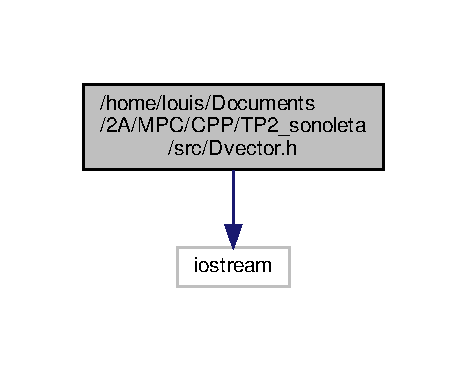
\includegraphics[width=156pt]{_dvector_8h__incl}
\end{center}
\end{figure}
\subsection*{Classes}
\begin{DoxyCompactItemize}
\item 
class \hyperlink{class_dvector}{Dvector}
\end{DoxyCompactItemize}


\subsection{Description détaillée}
classe vecteur de base, peut stocker des nombres au format double 
%--- End generated contents ---

% Index
\backmatter
\newpage
\phantomsection
\clearemptydoublepage
\addcontentsline{toc}{chapter}{Index}
\printindex

\end{document}
